\newcommand\version{v2}
\problemname{Kungarikesuppdelning}
I ett fjärran kungarike finns $N$ städer numrerade från $0$ till $N-1$.
Städerna är anslutna till varandra med $N-1$ gator som går att använda i båda riktningarna.
Alla gator är lika långa och ansluter exakt två städer på ett sådant sätt att det finns en unik väg mellan alla par av städer.

Tyvärr har den gamla kungen dött, utan att utse en efterträdare. Detta ledde till ett inbördeskrig mellan rikets $P$ grevar (numrerade från $0$ till $P - 1$) som alla ville ha kontroll över riket.

Efter ett långt och hemskt krig insåg grevarna att ingen ensam greve kunde vinna kriget. De gick med på ett fredsavtal, där riket delas upp i $P$ delar, en per greve. Delarna måste vara så att om två städer $a$ och $b$ tillhör samma greve, så måste alla städer på den unika vägen mellan $a$ och $b$ också tillhöra greven. Eftersom ingen greve vill lämnas maktlös måste varje greve få minst en stad.

Ingen greve vill heller få mindre än någon annan, så det totala värdet av alla städer måste vara detsamma för varje greve. Det totala värdet är summan av varje stads värde.

\section*{Exempel}
Låt kungariket ha $N = 5$ städer, anslutna av gator som i figuren:
\begin{figure}[h!]
  \centering
  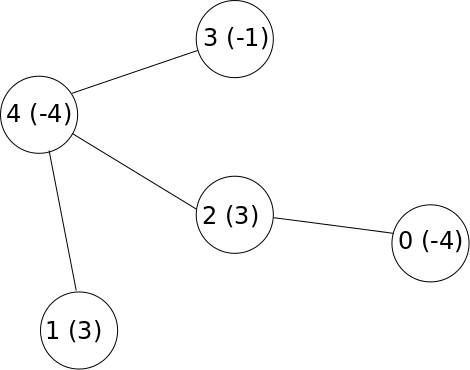
\includegraphics[width=0.3\textwidth]{sample.png}
  \caption{Illustration av exemplet}
\end{figure}
Varje stad har ett värde, givet inom paranteser efter stadens nummer.

Vi vill dela in riket i $P = 3$ delar.
En möjlig indelning är $(0, 2)$, $(3)$, $(1, 4)$.
Varje dels värde blir då $-4 + 3 = -1$, $-1$, och $3 - 4 = -1$,
så alla delar i denna uppdelning har samma värde.

Notera att $(0, 1)$ $(3)$, $(2, 4)$ inte är en giltig uppdelning trots att varje del har samma värde.
Detta är för att vägen mellan städerna $0$ och $1$ består av $1, 4, 2, 0$, men städerna $4$ och $2$ tillhör en annan greve.

\section*{Uppgift}
Uppgiften är att beräkna en uppdelning av kungariket som beskriven. Du ska implementera funktionen
\texttt{division(N, P, C, F, T)}.

\begin{itemize}
  \item \texttt{division(N, P, C, F, T)} - denna funktion kommer anropas exakt en gång av domaren.
  \begin{itemize}
    \item \texttt{N}: antalet städer i kungariket.
    \item \texttt{P}: antalet delar vi vill dela in kungariket i.
    \item \texttt{C}: en array med $N$ element. \texttt{C[i]} ($0 \le i < N$) innehåller den $i$:te stadens värde.
    \item \texttt{F}: en array med $N - 1$ element. \texttt{F[i]} ($0 \le i < N - 1$) innehåller den ena staden som den $i$:te vägen går mellan.
    \item \texttt{T}: en array med $N - 1$ element. \texttt{T[i]} ($0 \le i < N - 1$) innehåller den andra staden som den $i$:te vägen går mellan.
    \item Det är alltid möjligt att resa mellan varje par av städer med någon sekvens av vägar.
    \item $|C[i]| < 10^9$
    \item Funktionen ska returnera 1 om det existerar en sådan indelning, och 0 om det är omöjligt.
  \end{itemize}
\end{itemize}

Dessutom ska du göra exakt ett anrop till \texttt{parts(S)} för att konstruera din indelning.
\begin{itemize}
  \item \texttt{parts(S)} - denna funktion ska anropas exakt en gång.
  \begin{itemize}
    \item \texttt{S}: en array med $N$ element. $S[i]$ $(0 \le i < N)$ ska innehålla numret på den greve som får den $i$:te staden.
    \item Denna funktion har inget returvärde.
  \end{itemize}
\end{itemize}


\section*{Delpoäng}
Problemet består av flera grupper av testfall. Varje grupp ger ett visst antal poäng och för att klara det måste du klara alla testfall i gruppen.

\begin{tabular}{|l|l|l|}
  \hline
  \textbf{Grupp} & \textbf{Poäng} & \textbf{Gränser} \\ \hline
  1 & 8 & $P = 2 \le N \le 1\,000$ \\ \hline
  2 & 10 & $1 \le P \le N \le 1\,000$, $C[i] > 0$ \\ \hline
  3 & 16 & $1 \le P \le N \le 1\,000$, bara städerna $i$ och $i + 1$ har vägar (för $0 \le i < N - 1$). \\ \hline
  4 & 18 & $1 \le P \le N \le 1\,000$ \\ \hline
  5 & 18 & $1 \le P \le N \le 100\,000$, $C[i] > 0$ \\ \hline
  6 & 30 & $1 \le P \le N \le 100\,000$ \\ \hline
\end{tabular}

\section*{Indataformat}
Exempeldomaren läser indata i följande format:

\begin{itemize}
  \item line $1$: \texttt{N P}
  \item line $2$: \texttt{C[0] C[1] .. C[N - 1]}
  \item line $3$: \texttt{F[0] F[1] .. F[N - 2]}
  \item line $4$: \texttt{T[0] T[1] .. T[N - 2]}
\end{itemize}

\section*{Utdataformat}
Exempeldomaren skriver först ut en rad med värdet som returnerades av \texttt{division(N, P, C, F, T)}.
Nästas rad innehåller de $N$ heltalen som gavs i anropet till \texttt{parts(R)}.

